% Options for packages loaded elsewhere
\PassOptionsToPackage{unicode}{hyperref}
\PassOptionsToPackage{hyphens}{url}
\PassOptionsToPackage{dvipsnames,svgnames,x11names}{xcolor}
%
\documentclass[
  letterpaper,
  DIV=11,
  numbers=noendperiod]{scrartcl}

\usepackage{amsmath,amssymb}
\usepackage{iftex}
\ifPDFTeX
  \usepackage[T1]{fontenc}
  \usepackage[utf8]{inputenc}
  \usepackage{textcomp} % provide euro and other symbols
\else % if luatex or xetex
  \usepackage{unicode-math}
  \defaultfontfeatures{Scale=MatchLowercase}
  \defaultfontfeatures[\rmfamily]{Ligatures=TeX,Scale=1}
\fi
\usepackage{lmodern}
\ifPDFTeX\else  
    % xetex/luatex font selection
\fi
% Use upquote if available, for straight quotes in verbatim environments
\IfFileExists{upquote.sty}{\usepackage{upquote}}{}
\IfFileExists{microtype.sty}{% use microtype if available
  \usepackage[]{microtype}
  \UseMicrotypeSet[protrusion]{basicmath} % disable protrusion for tt fonts
}{}
\makeatletter
\@ifundefined{KOMAClassName}{% if non-KOMA class
  \IfFileExists{parskip.sty}{%
    \usepackage{parskip}
  }{% else
    \setlength{\parindent}{0pt}
    \setlength{\parskip}{6pt plus 2pt minus 1pt}}
}{% if KOMA class
  \KOMAoptions{parskip=half}}
\makeatother
\usepackage{xcolor}
\setlength{\emergencystretch}{3em} % prevent overfull lines
\setcounter{secnumdepth}{5}
% Make \paragraph and \subparagraph free-standing
\ifx\paragraph\undefined\else
  \let\oldparagraph\paragraph
  \renewcommand{\paragraph}[1]{\oldparagraph{#1}\mbox{}}
\fi
\ifx\subparagraph\undefined\else
  \let\oldsubparagraph\subparagraph
  \renewcommand{\subparagraph}[1]{\oldsubparagraph{#1}\mbox{}}
\fi


\providecommand{\tightlist}{%
  \setlength{\itemsep}{0pt}\setlength{\parskip}{0pt}}\usepackage{longtable,booktabs,array}
\usepackage{calc} % for calculating minipage widths
% Correct order of tables after \paragraph or \subparagraph
\usepackage{etoolbox}
\makeatletter
\patchcmd\longtable{\par}{\if@noskipsec\mbox{}\fi\par}{}{}
\makeatother
% Allow footnotes in longtable head/foot
\IfFileExists{footnotehyper.sty}{\usepackage{footnotehyper}}{\usepackage{footnote}}
\makesavenoteenv{longtable}
\usepackage{graphicx}
\makeatletter
\def\maxwidth{\ifdim\Gin@nat@width>\linewidth\linewidth\else\Gin@nat@width\fi}
\def\maxheight{\ifdim\Gin@nat@height>\textheight\textheight\else\Gin@nat@height\fi}
\makeatother
% Scale images if necessary, so that they will not overflow the page
% margins by default, and it is still possible to overwrite the defaults
% using explicit options in \includegraphics[width, height, ...]{}
\setkeys{Gin}{width=\maxwidth,height=\maxheight,keepaspectratio}
% Set default figure placement to htbp
\makeatletter
\def\fps@figure{htbp}
\makeatother
\newlength{\cslhangindent}
\setlength{\cslhangindent}{1.5em}
\newlength{\csllabelwidth}
\setlength{\csllabelwidth}{3em}
\newlength{\cslentryspacingunit} % times entry-spacing
\setlength{\cslentryspacingunit}{\parskip}
\newenvironment{CSLReferences}[2] % #1 hanging-ident, #2 entry spacing
 {% don't indent paragraphs
  \setlength{\parindent}{0pt}
  % turn on hanging indent if param 1 is 1
  \ifodd #1
  \let\oldpar\par
  \def\par{\hangindent=\cslhangindent\oldpar}
  \fi
  % set entry spacing
  \setlength{\parskip}{#2\cslentryspacingunit}
 }%
 {}
\usepackage{calc}
\newcommand{\CSLBlock}[1]{#1\hfill\break}
\newcommand{\CSLLeftMargin}[1]{\parbox[t]{\csllabelwidth}{#1}}
\newcommand{\CSLRightInline}[1]{\parbox[t]{\linewidth - \csllabelwidth}{#1}\break}
\newcommand{\CSLIndent}[1]{\hspace{\cslhangindent}#1}

\usepackage{booktabs}
\usepackage{longtable}
\usepackage{array}
\usepackage{multirow}
\usepackage{wrapfig}
\usepackage{float}
\usepackage{colortbl}
\usepackage{pdflscape}
\usepackage{tabu}
\usepackage{threeparttable}
\usepackage{threeparttablex}
\usepackage[normalem]{ulem}
\usepackage{makecell}
\usepackage{xcolor}
\KOMAoption{captions}{tableheading}
\makeatletter
\makeatother
\makeatletter
\makeatother
\makeatletter
\@ifpackageloaded{caption}{}{\usepackage{caption}}
\AtBeginDocument{%
\ifdefined\contentsname
  \renewcommand*\contentsname{Table of contents}
\else
  \newcommand\contentsname{Table of contents}
\fi
\ifdefined\listfigurename
  \renewcommand*\listfigurename{List of Figures}
\else
  \newcommand\listfigurename{List of Figures}
\fi
\ifdefined\listtablename
  \renewcommand*\listtablename{List of Tables}
\else
  \newcommand\listtablename{List of Tables}
\fi
\ifdefined\figurename
  \renewcommand*\figurename{Figure}
\else
  \newcommand\figurename{Figure}
\fi
\ifdefined\tablename
  \renewcommand*\tablename{Table}
\else
  \newcommand\tablename{Table}
\fi
}
\@ifpackageloaded{float}{}{\usepackage{float}}
\floatstyle{ruled}
\@ifundefined{c@chapter}{\newfloat{codelisting}{h}{lop}}{\newfloat{codelisting}{h}{lop}[chapter]}
\floatname{codelisting}{Listing}
\newcommand*\listoflistings{\listof{codelisting}{List of Listings}}
\makeatother
\makeatletter
\@ifpackageloaded{caption}{}{\usepackage{caption}}
\@ifpackageloaded{subcaption}{}{\usepackage{subcaption}}
\makeatother
\makeatletter
\@ifpackageloaded{tcolorbox}{}{\usepackage[skins,breakable]{tcolorbox}}
\makeatother
\makeatletter
\@ifundefined{shadecolor}{\definecolor{shadecolor}{rgb}{.97, .97, .97}}
\makeatother
\makeatletter
\makeatother
\makeatletter
\makeatother
\ifLuaTeX
  \usepackage{selnolig}  % disable illegal ligatures
\fi
\IfFileExists{bookmark.sty}{\usepackage{bookmark}}{\usepackage{hyperref}}
\IfFileExists{xurl.sty}{\usepackage{xurl}}{} % add URL line breaks if available
\urlstyle{same} % disable monospaced font for URLs
\hypersetup{
  pdftitle={Jean Pockets and Gender},
  pdfauthor={Hari Lee Robledo},
  colorlinks=true,
  linkcolor={blue},
  filecolor={Maroon},
  citecolor={Blue},
  urlcolor={Blue},
  pdfcreator={LaTeX via pandoc}}

\title{Jean Pockets and Gender\thanks{Code and data are available at:
https://github.com/hari-lr/pockets-and-gender}}
\usepackage{etoolbox}
\makeatletter
\providecommand{\subtitle}[1]{% add subtitle to \maketitle
  \apptocmd{\@title}{\par {\large #1 \par}}{}{}
}
\makeatother
\subtitle{subtitle}
\author{Hari Lee Robledo}
\date{April 23, 2024}

\begin{document}
\maketitle
\begin{abstract}
Fashion has long reflected and reinforced gender inequalities, with
women's clothing often lacking functional pockets found in men's
garments. A 2018 study by Jan Diehm \& Amber Thomas on The Pudding
revealed this discrepancy, highlighting inferior pocket functionality in
women's jeans. This paper aims to reproduce these findings and explore
if gender disparities extend to pricing. Using the same data, we analyze
the correlation between prices of men's and women's jeans. Results
suggest that women's jeans not only have smaller pockets but also tend
to be more expensive. This study sheds light on gender inequalities in
everyday products and their broader implications. {[}UPDATE according to
findingsThe findings revealed that pocket area alone may not be a strong
predictor of jeans prices for either gender, and there may be other
factors influencing the pricing of jeans.{]}
\end{abstract}
\ifdefined\Shaded\renewenvironment{Shaded}{\begin{tcolorbox}[sharp corners, borderline west={3pt}{0pt}{shadecolor}, interior hidden, frame hidden, enhanced, boxrule=0pt, breakable]}{\end{tcolorbox}}\fi

\renewcommand*\contentsname{Table of contents}
{
\hypersetup{linkcolor=}
\setcounter{tocdepth}{3}
\tableofcontents
}
\newpage

\hypertarget{introduction}{%
\section{Introduction}\label{introduction}}

Throughout history, women have faced numerous restrictions and
limitations, often ingrained within societal norms and cultural
practices. Among these limitations, the realm of fashion has served as
both a reflection and an enforcer of gender-based inequalities. From
ancient times to the modern era, clothing has been a means of expressing
social status, cultural identity, and gender roles. According to design
expert, Hannah Carlson, pocket inequality stems from the way clothes are
designed and made, she explains that: ``From a very early age, I think
we sort of agree as a culture that womenswear, girlswear is meant to be
pretty,'' she said. ``And menswear, boyswear is meant to be
utilitarian'' (Alwahaidi 2018). Men's garments historically incorporated
functional pockets, allowing them to carry essentials such as money,
keys, and tools, women's clothing has often lacked this practical
feature. Instead, women's garments have frequently been designed with
form-fitting silhouettes, delicate fabrics, and ornamental details,
prioritizing aesthetics over utility.However, the 1880s, women began to
be vocal about pocket inequality, as the ``demand for the vote and the
demand for pockets were made together'' (Alwahaidi 2018).

In 2018, Jan Diehm \& Amber Thomas published Womens´s Pockets are
Inferior on \emph{The Pudding}, a data-centric digital publication. In
this paper, they ``measured pockets in both men´s and women's pants in
20 of the US' most popular blue jeans brands'' (Jan Diehm 2018). They
``programmatically determined whether various everyday items could fit
in an otherwise empty pocket in jeans that aren't being worn'' (Jan
Diehm 2018)., and concluded that women´s pockets were less functional
than men´s.

Using the data from the previously described article, this paper will
graphically reproduce the results and examine whether there is a
correlation between the prices of men's jeans and women's jeans. The
study seeks to determine if women's jeans not only have smaller and less
functional pockets but also tend to be more expensive. This will help
better understand if gender inequality is only reflected in the jean's
pockets or in pricing as well. A linear regression analysis revealed
divergent findings regarding the relationship between pocket area and
price in men's and women's jeans. For men's jeans, no significant
correlation was found between pocket area and price, indicating that
changes in pocket size do not significantly affect the price of men's
jeans. In contrast, although a negative correlation was observed in
women's jeans, it was not statistically significant, suggesting that
while larger pocket areas might be associated with slightly lower
prices, other factors likely play a more influential role in determining
the price of women's jeans.

This paper is structured into the following sections: Data, which
explains the collection and cleaning process; Results, presenting trends
and correlations found in the data; Discussion, comparing and evaluating
the data; and Conclusion, summarizing the findings.

\hypertarget{data}{%
\section{Data}\label{data}}

The data utilized in this paper was retrieved from The Pudding GitHub
Site Portal, specifically the data collected by Jan Diehm and Amber
Thomas (Jan Diehm 2018). Data was collected, cleaned, and analyzed using
the open-source statistical programming software R (R Core Team 2023).
This process involved various packages within R, including
\texttt{tidyverse} (Wickham et al. 2019), \texttt{jsonlite} (Ooms 2014),
\texttt{readr} (Wickham, Hester, and Bryan 2024), \texttt{janitor}
(Firke 2021), \texttt{dplyr} (Wickham et al. 2023), \texttt{tibble}
(Müller and Wickham 2023), \texttt{ggplot2} (Wickham 2016),
\texttt{knitr} (Xie 2024), and \texttt{kableExtra} (Zhu 2021). A
comprehensive description of the data gathering and cleaning process is
provided in the following subsections.

\hypertarget{dataset}{%
\subsection{Dataset}\label{dataset}}

In the original study, researchers examined jean pocket sizes across 20
brands, encompassing both men's and women's jeans, including skinny and
straight styles. The assessment involved scrutinizing four pairs of
jeans per brand, all tailored with a 32-inch waistband, despite falling
below the median waist size for women in the US. Measurements were
meticulously taken in physical stores located in Nashville, New York,
and Seattle, with pocket dimensions recorded while jeans were unbuttoned
and unzipped, from the inside (Jan Diehm 2018). The study incorporated
computer-generated images to illustrate pocket curvature. Various
objects, such as standard pen sizes and a front pocket wallet, were
utilized to evaluate pocket compatibility. Additionally, area
measurements were computed using the \texttt{d3.polygonArea()} function
in d3.v4, offering valuable insights into the spatial characteristics of
the jean pockets. These methods were intended to give a complete
understanding of jean pocket sizes and how well they can hold everyday
items. (Jan Diehm 2018).

In this paper, the dataset used for analysis was obtained from
\texttt{measurementRectangles.json}. This dataset mirrors the
measurements found in \texttt{measurements.csv}, including brand, style,
gender specification (men or women), product name, brand size, waist
size, fabric composition, price, and height and width measurements of
jean pockets (see Table~\ref{tbl-raw_data}). Notably, the dataset
contains a ``pocketArea'' column representing the area of the polygon
generated from a pocket's measurements. However, it's important to note
that the units of measurement for this area are not explicitly specified
in the provided metadata. To determine the units, one must examine how
the measurements were collected and processed. Since the measurements
were processed using computer-generated calculations and intended for
web display, it is possible that the pocket area is denoted in square
centimeters (px²). However, without explicit confirmation from the data
documentation or creators of the dataset, absolute certainty regarding
the units of measurement remains elusive.

\hypertarget{tbl-raw_data}{}
\begin{longtable}[]{@{}
  >{\raggedright\arraybackslash}p{(\columnwidth - 10\tabcolsep) * \real{0.1748}}
  >{\centering\arraybackslash}p{(\columnwidth - 10\tabcolsep) * \real{0.0971}}
  >{\centering\arraybackslash}p{(\columnwidth - 10\tabcolsep) * \real{0.1068}}
  >{\centering\arraybackslash}p{(\columnwidth - 10\tabcolsep) * \real{0.1650}}
  >{\centering\arraybackslash}p{(\columnwidth - 10\tabcolsep) * \real{0.3883}}
  >{\raggedright\arraybackslash}p{(\columnwidth - 10\tabcolsep) * \real{0.0680}}@{}}
\caption{\label{tbl-raw_data}Sample of Raw Jean Pockets
Data}\tabularnewline
\toprule\noalign{}
\begin{minipage}[b]{\linewidth}\raggedright
Brand
\end{minipage} & \begin{minipage}[b]{\linewidth}\centering
Style
\end{minipage} & \begin{minipage}[b]{\linewidth}\centering
Men/Women
\end{minipage} & \begin{minipage}[b]{\linewidth}\centering
Name
\end{minipage} & \begin{minipage}[b]{\linewidth}\centering
Fabric
\end{minipage} & \begin{minipage}[b]{\linewidth}\raggedright
Price
\end{minipage} \\
\midrule\noalign{}
\endfirsthead
\toprule\noalign{}
\begin{minipage}[b]{\linewidth}\raggedright
Brand
\end{minipage} & \begin{minipage}[b]{\linewidth}\centering
Style
\end{minipage} & \begin{minipage}[b]{\linewidth}\centering
Men/Women
\end{minipage} & \begin{minipage}[b]{\linewidth}\centering
Name
\end{minipage} & \begin{minipage}[b]{\linewidth}\centering
Fabric
\end{minipage} & \begin{minipage}[b]{\linewidth}\raggedright
Price
\end{minipage} \\
\midrule\noalign{}
\endhead
\bottomrule\noalign{}
\endlastfoot
7 for All Mankind & straight & men & The Straight & 98\% cotton, 2\%
spandex & 179.00 \\
7 for All Mankind & skinny & men & Paxtyn & 92\% cotton, 6\% polyester,
2\% spandex & 209.00 \\
Abercrombie & slim & men & Langdon Slim & 95\% cotton, 4\% polyester,
1\% elastane & 78.00 \\
Abercrombie & straight & men & Kennan Straight & 95\% cotton, 4\%
polyester, 1\% elastane & 78.00 \\
American Eagle & straight & men & Straight & 85\% cotton, 13\%
polyester, 2\% elastane & 49.95 \\
\end{longtable}

\hypertarget{data-cleaning}{%
\subsection{Data Cleaning}\label{data-cleaning}}

Initially, the code read the JSON data containing pocket area
measurements, standardized the column names using the
\texttt{clean\_names()} function, and stored the cleaned data in the
\texttt{cleaned\_area\_data} dataframe. Subsequently, the data was
filtered based on gender, separating jeans intended for women and men
using the \texttt{filter()} function. Only the ``price'' and
``pocket\_area'' columns were retained for further analysis in the
resulting dataframes \texttt{men\_jeans\_data} and
\texttt{women\_jeans\_data} (see Table~\ref{tbl-menwomen_table}),
respectively. In the final step, the cleaned data was saved into CSV
files. The \texttt{write.csv()} function was utilized to export the
data, with separate CSV files generated for women's and men's jeans.

\begin{table}

\caption{\label{tbl-menwomen_table}Sample of Cleaned
Men\textquotesingle s and Women´s
Data}\begin{minipage}[t]{0.50\linewidth}
\subcaption{\label{tbl-menwomen_table-1}Men's Data}

{\centering 

\begin{tabular}[t]{rr}
\toprule
Price & Pocket Area\\
\midrule
179.00 & 11222.73\\
209.00 & 10841.94\\
78.00 & 10624.65\\
78.00 & 10134.15\\
49.95 & 10555.40\\
\bottomrule
\end{tabular}

}

\end{minipage}%
%
\begin{minipage}[t]{0.50\linewidth}
\subcaption{\label{tbl-menwomen_table-2}Women's Data}

{\centering 

\begin{tabular}[t]{rr}
\toprule
Price & Pocket Area\\
\midrule
199.00 & 5557.218\\
159.00 & 5811.112\\
78.00 & 8757.578\\
88.00 & 9688.483\\
39.95 & 6408.587\\
\bottomrule
\end{tabular}

}

\end{minipage}%

\end{table}

To visually explore the relationship between pocket area and price for
both men's (see Figure~\ref{fig-price_per_pocket_men}) and women's jeans
(see Figure~\ref{fig-price_per_pocket_women}), scatter plots with
regression lines were created.

\begin{figure}

{\centering 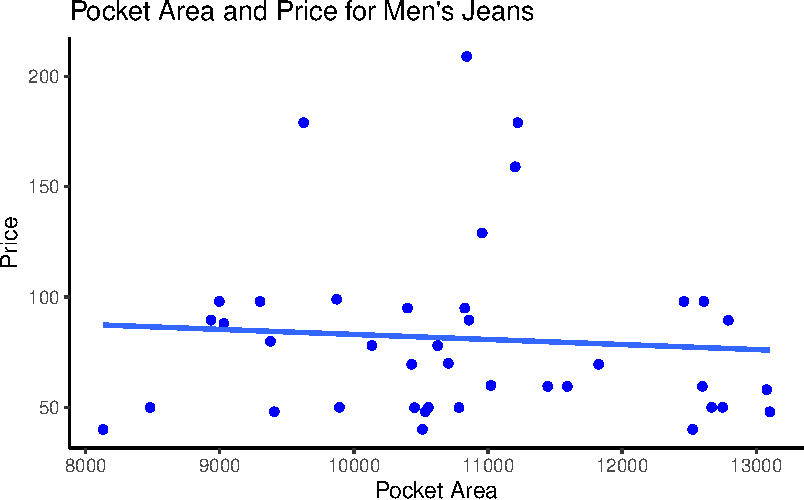
\includegraphics{paper_files/figure-pdf/fig-price_per_pocket_men-1.pdf}

}

\caption{\label{fig-price_per_pocket_men}Jean Price vs Pocket Size
(Men)}

\end{figure}

\begin{figure}

{\centering 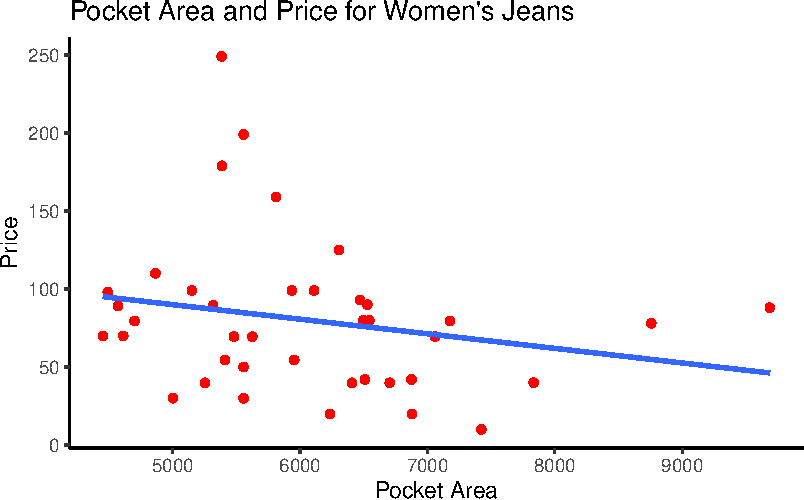
\includegraphics{paper_files/figure-pdf/fig-price_per_pocket_women-1.pdf}

}

\caption{\label{fig-price_per_pocket_women}Jean Price vs Pocket Size
(Women)}

\end{figure}

These plots visually depict the relationship between pocket area and
price for men's and women's jeans. Additionally, to compute the standard
deviation of price for both men's and women's jeans, the \texttt{sd()}
function can be applied to the respective columns in the
\texttt{men\_jeans\_data} and \texttt{women\_jeans\_data} dataframes.
The standard deviation of price for women's jeans is 48.79, while for
men's jeans, it is 40.49, indicating the variability in prices within
each gender category. This measure helps assess the spread of prices
around the mean and provides insight into the degree of dispersion in
price values among the observed jeans.

\hypertarget{model}{%
\section{Model}\label{model}}

To gain further insights and make predictions about {[}{]}, we will be
implementing a linear regression model.

The final model is displayed here.

\[L = \beta_0 + \beta_1S + \epsilon\]

Where:

\begin{itemize}
\tightlist
\item
  \(L\) represents the dependent variable, which is the overall price of
  jeans
\item
  \(S\) represents the independent variable, which is the pocket area
\item
  \(\beta_0\) represents the intercept of the regression line, which is
  the predicted value of \(L\) when \(S\) is equal to zero
\item
  \(\beta_1\) represents the slope of the regression line, which is the
  change in \(L\) for a one-unit increase in \(S\)
\item
  \(\epsilon\) represents the random error term, which accounts for
  variability in \(L\) that is not explained by the relationship with
  \(S\)
\end{itemize}

Linear regression seeks to determine the optimal parameters \(\beta_0\)
and \(\beta_1\) that minimize the discrepancies between predicted and
observed prices across varying pocket areas in the dataset. Through this
minimization process, the model constructs a line that most accurately
represents the association between pocket area and price. Consequently,
we can predict price values based on known pocket area measurements.
This regression analysis sheds light on how pocket area influences the
pricing of jeans for both men and women, offering valuable insights into
the pricing dynamics within each gender category.

\hypertarget{results}{%
\section{Results}\label{results}}

\hypertarget{tbl-men_model_summary}{}
\begin{table}

\caption{\label{tbl-men_model_summary}Summary of Linear Regression Model for Men's Jeans }Summary of Linear Regression Model for Men's Jeans}
\centering
\begin{tabular}[t]{l|c|c|c|c}
\hline
  & Estimate & Std. Error & t value & Pr(>|t|)\\
\hline
(Intercept) & 105.9002168 & 53.5254438 & 1.9785024 & 0.0551543\\
\hline
pocket\_area & -0.0022856 & 0.0049134 & -0.4651738 & 0.6444619\\
\hline
\end{tabular}
\end{table}

\hypertarget{tbl-women_model_summary}{}
\begin{table}

\caption{\label{tbl-women_model_summary}Summary of Linear Regression Model for Women's Jeans }Summary of Linear Regression Model for Women's Jeans}
\centering
\begin{tabular}[t]{l|c|c|c|c}
\hline
  & Estimate & Std. Error & t value & Pr(>|t|)\\
\hline
(Intercept) & 136.7159600 & 42.0324855 & 3.252626 & 0.0024018\\
\hline
pocket\_area & -0.0093445 & 0.0068483 & -1.364495 & 0.1804384\\
\hline
\end{tabular}
\end{table}

A scatterplot was generated to compare pocket area and price for both
men's and women's jeans. Each gender category was represented by a
distinct color in the plot. Additionally, linear regression lines were
overlaid for each gender group to observe potential differences in the
relationship between pocket area and price.

This visualization facilitated the comparison of how pocket area related
to price for men's and women's jeans separately. By including separate
regression lines for each gender, we could assess the direction and
strength of the relationship between these variables within each group.
The use of different colors for men and women aided in distinguishing
between the two groups, enabling easy interpretation of the plot.

\begin{figure}

{\centering 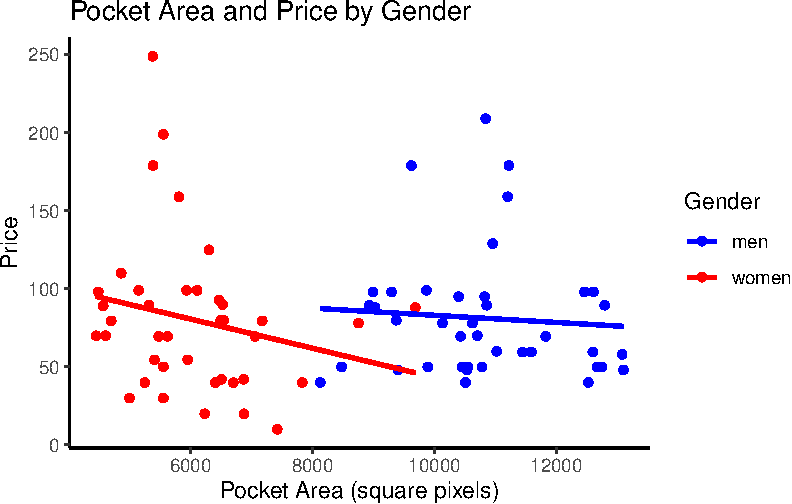
\includegraphics{paper_files/figure-pdf/fig-price_per_pocket_gender-1.pdf}

}

\caption{\label{fig-price_per_pocket_gender}Jean Price vs.~Pocket Area
Size per Gender}

\end{figure}

After visualizing the linear regression for both men's and women's
jeans, I proceeded to analyze the results obtained from the regression
models:

The linear regression models for both men's and women's jeans revealed
interesting insights into the relationship between pocket area and
price.

For men's jeans, the coefficient estimate for pocket area (\(\beta_1\))
is -0.002286, indicating a very small and statistically insignificant
negative association between pocket area and price. This suggests that,
on average, changes in pocket area do not have a significant impact on
the price of men's jeans. The p-value associated with the pocket area
coefficient is 0.6445, which is much greater than the typical
significance level of 0.05. Additionally, the ( R\^{}2 ) value, which
measures the proportion of variance in the dependent variable explained
by the independent variable, is very low at 0.005662. Overall, these
results suggest that there is little evidence to suggest a meaningful
relationship between pocket area and price for men's jeans.

In contrast, for women's jeans, the coefficient estimate for pocket area
is -0.009345, also indicating a small negative association with price,
although it is slightly larger in magnitude compared to men's jeans.
However, like men's jeans, this coefficient is statistically
insignificant with a p-value of 0.1804. The ( R\^{}2 ) value for women's
jeans is slightly higher at 0.04671, indicating that pocket area
explains a slightly larger proportion of the variance in price compared
to men's jeans. Despite this, the overall relationship between pocket
area and price remains weak for women's jeans.

In summary, the results suggest that pocket area is not a significant
predictor of price for either men's or women's jeans in the dataset
analyzed. Other factors not considered in this analysis are likely to
have a greater influence on the pricing of jeans for both genders.

\hypertarget{discussion}{%
\section{Discussion}\label{discussion}}

\hypertarget{sec-first-point}{%
\subsection{First discussion point}\label{sec-first-point}}

\hypertarget{second-discussion-point}{%
\subsection{Second discussion point}\label{second-discussion-point}}

\hypertarget{third-discussion-point}{%
\subsection{Third discussion point}\label{third-discussion-point}}

\#\#Weaknesses and next steps

\newpage

\appendix

\hypertarget{appendix}{%
\section*{Appendix}\label{appendix}}
\addcontentsline{toc}{section}{Appendix}

\newpage

\hypertarget{references}{%
\section*{References}\label{references}}
\addcontentsline{toc}{section}{References}

\hypertarget{refs}{}
\begin{CSLReferences}{1}{0}
\leavevmode\vadjust pre{\hypertarget{ref-carlson}{}}%
Alwahaidi, Keena. 2018. \emph{Women's Apparel Doesn't Have Enough
Pockets. This Expert Says That Has to Change}.

\leavevmode\vadjust pre{\hypertarget{ref-janitor}{}}%
Firke, Sam. 2021. \emph{Janitor: Simple Tools for Examining and Cleaning
Dirty Data}. \url{https://github.com/sfirke/janitor}.

\leavevmode\vadjust pre{\hypertarget{ref-pudding}{}}%
Jan Diehm, Amber Thomas. 2018. \emph{Womens´s Pockets Are Inferior}.

\leavevmode\vadjust pre{\hypertarget{ref-tibble}{}}%
Müller, Kirill, and Hadley Wickham. 2023. \emph{Tibble: Simple Data
Frames}. \url{https://tibble.tidyverse.org/}.

\leavevmode\vadjust pre{\hypertarget{ref-jsonlite}{}}%
Ooms, Jeroen. 2014. {``The Jsonlite Package: A Practical and Consistent
Mapping Between JSON Data and r Objects.''} \emph{arXiv:1403.2805
{[}Stat.CO{]}}. \url{https://arxiv.org/abs/1403.2805}.

\leavevmode\vadjust pre{\hypertarget{ref-citeR}{}}%
R Core Team. 2023. \emph{R: A Language and Environment for Statistical
Computing}. Vienna, Austria: R Foundation for Statistical Computing.
\url{https://www.R-project.org/}.

\leavevmode\vadjust pre{\hypertarget{ref-ggplot2}{}}%
Wickham, Hadley. 2016. \emph{Ggplot2: Elegant Graphics for Data
Analysis}. Springer-Verlag New York.
\url{https://ggplot2.tidyverse.org}.

\leavevmode\vadjust pre{\hypertarget{ref-tidyverse}{}}%
Wickham, Hadley, Mara Averick, Jennifer Bryan, Winston Chang, Lucy
D'Agostino McGowan, Romain François, Garrett Grolemund, et al. 2019.
{``Welcome to the {tidyverse}.''} \emph{Journal of Open Source Software}
4 (43): 1686. \url{https://doi.org/10.21105/joss.01686}.

\leavevmode\vadjust pre{\hypertarget{ref-dplyr}{}}%
Wickham, Hadley, Romain François, Lionel Henry, Kirill Müller, and Davis
Vaughan. 2023. \emph{Dplyr: A Grammar of Data Manipulation}.

\leavevmode\vadjust pre{\hypertarget{ref-readr}{}}%
Wickham, Hadley, Jim Hester, and Jennifer Bryan. 2024. \emph{Readr: Read
Rectangular Text Data}. \url{https://readr.tidyverse.org}.

\leavevmode\vadjust pre{\hypertarget{ref-knitr}{}}%
Xie, Yihui. 2024. \emph{Knitr: A General-Purpose Package for Dynamic
Report Generation in r}. \url{https://yihui.org/knitr/}.

\leavevmode\vadjust pre{\hypertarget{ref-kableExtra}{}}%
Zhu, Hao. 2021. \emph{kableExtra: Construct Complex Table with 'Kable'
and Pipe Syntax}.

\end{CSLReferences}



\end{document}
